% Graphic for TeX using PGF
% Title: /home/di3go/workspace/t02-core-musa/doc/architecture/pictures/diagrams/pc.dia
% Creator: Dia v0.97.3
% CreationDate: Tue Dec 16 22:39:35 2014
% For: di3go
% \usepackage{tikz}
% The following commands are not supported in PSTricks at present
% We define them conditionally, so when they are implemented,
% this pgf file will use them.
\ifx\du\undefined
  \newlength{\du}
\fi
\setlength{\du}{15\unitlength}
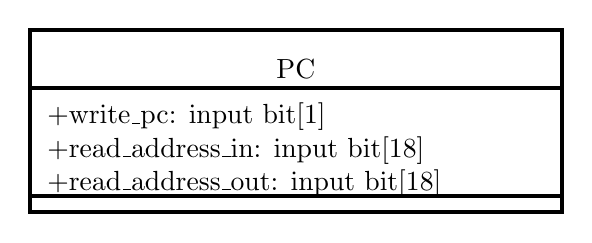
\begin{tikzpicture}
\pgftransformxscale{1.000000}
\pgftransformyscale{-1.000000}
\definecolor{dialinecolor}{rgb}{0.000000, 0.000000, 0.000000}
\pgfsetstrokecolor{dialinecolor}
\definecolor{dialinecolor}{rgb}{1.000000, 1.000000, 1.000000}
\pgfsetfillcolor{dialinecolor}
\pgfsetlinewidth{0.100000\du}
\pgfsetdash{}{0pt}
\definecolor{dialinecolor}{rgb}{1.000000, 1.000000, 1.000000}
\pgfsetfillcolor{dialinecolor}
\fill (-9.998130\du,-11.940600\du)--(-9.998130\du,-10.540600\du)--(2.821870\du,-10.540600\du)--(2.821870\du,-11.940600\du)--cycle;
\definecolor{dialinecolor}{rgb}{0.000000, 0.000000, 0.000000}
\pgfsetstrokecolor{dialinecolor}
\draw (-9.998130\du,-11.940600\du)--(-9.998130\du,-10.540600\du)--(2.821870\du,-10.540600\du)--(2.821870\du,-11.940600\du)--cycle;
% setfont left to latex
\definecolor{dialinecolor}{rgb}{0.000000, 0.000000, 0.000000}
\pgfsetstrokecolor{dialinecolor}
\node at (-3.588130\du,-10.990600\du){PC};
\definecolor{dialinecolor}{rgb}{1.000000, 1.000000, 1.000000}
\pgfsetfillcolor{dialinecolor}
\fill (-9.998130\du,-10.540600\du)--(-9.998130\du,-7.940600\du)--(2.821870\du,-7.940600\du)--(2.821870\du,-10.540600\du)--cycle;
\definecolor{dialinecolor}{rgb}{0.000000, 0.000000, 0.000000}
\pgfsetstrokecolor{dialinecolor}
\draw (-9.998130\du,-10.540600\du)--(-9.998130\du,-7.940600\du)--(2.821870\du,-7.940600\du)--(2.821870\du,-10.540600\du)--cycle;
% setfont left to latex
\definecolor{dialinecolor}{rgb}{0.000000, 0.000000, 0.000000}
\pgfsetstrokecolor{dialinecolor}
\node[anchor=west] at (-9.848130\du,-9.840600\du){+write\_pc: input bit\ensuremath{[}1\ensuremath{]}};
% setfont left to latex
\definecolor{dialinecolor}{rgb}{0.000000, 0.000000, 0.000000}
\pgfsetstrokecolor{dialinecolor}
\node[anchor=west] at (-9.848130\du,-9.040600\du){+read\_address\_in: input bit\ensuremath{[}18\ensuremath{]}};
% setfont left to latex
\definecolor{dialinecolor}{rgb}{0.000000, 0.000000, 0.000000}
\pgfsetstrokecolor{dialinecolor}
\node[anchor=west] at (-9.848130\du,-8.240600\du){+read\_address\_out: input bit\ensuremath{[}18\ensuremath{]}};
\definecolor{dialinecolor}{rgb}{1.000000, 1.000000, 1.000000}
\pgfsetfillcolor{dialinecolor}
\fill (-9.998130\du,-7.940600\du)--(-9.998130\du,-7.540600\du)--(2.821870\du,-7.540600\du)--(2.821870\du,-7.940600\du)--cycle;
\definecolor{dialinecolor}{rgb}{0.000000, 0.000000, 0.000000}
\pgfsetstrokecolor{dialinecolor}
\draw (-9.998130\du,-7.940600\du)--(-9.998130\du,-7.540600\du)--(2.821870\du,-7.540600\du)--(2.821870\du,-7.940600\du)--cycle;
\end{tikzpicture}
